\documentclass{standalone}
\usepackage{tikz}
\usepackage{ctex,siunitx}
\usepackage{tkz-euclide}
\usepackage{amsmath}
\usetikzlibrary{patterns, calc}
\usetikzlibrary {decorations.pathmorphing, decorations.pathreplacing, decorations.shapes,}
\begin{document}
\small
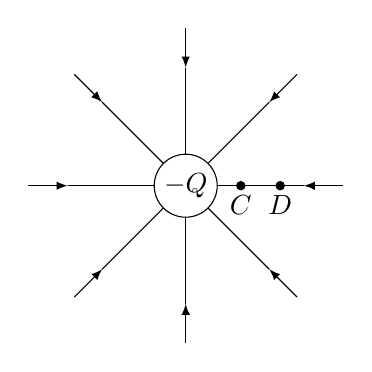
\begin{tikzpicture}[>=latex,scale=1.0]
  \foreach \x in {0,45,90,...,315}
	{
		\draw (0:0)--(\x: 1.5);
		\draw [<-](\x:1.5)--(\x: 2);
	}
	\draw (0,0) [fill=white] circle (.4);
	\draw (1.2,0) [fill=black] circle (1.5pt)node[below]{$D$};\draw (.7,0) [fill=black] circle (1.5pt)node[below]{$C$};
  \node at (0,0){$-Q$};
\end{tikzpicture}
\end{document}